\subsection{Vision Detection Principles}
% vision hardware set up + software implementation
In order to achieve the vision detection task we had broken down the task into 4 sub tasks as following
\begin{enumerate}
	\item Identify the Cards on the table.
	\item Coordinates and pose of the cards.
	\item Match the local coordinates to the world coordinates.
	\item Identify the features of the cards.
\end{enumerate}
	
Matlab image processing toolbox has been used for image processing tasks of this project. 

1.	Identify the cards on the table.
\begin{itemize}
	\item In the initial sweep after hiding the robot arm the camera will capture an image of the table. Histogram equalisation has been used to equalise the intensity over the image to make the image processing task easier. 
	\item The back of the card gives pixel values near to black colour in gray image. Using this data a logical image has been created by using a threshold of pixel values less than 0.09. After removing pixels areas less than 1000 using function; bwareopen a structured element has been used to morphologically close the founded blobs.
	\item •	The same logic has been used to find face up cards as well. In that threshold of 0.91 has been used as face ups are near to white colour.
\end{itemize}

\begin{figure}[position = here]
	\begin{centering}
		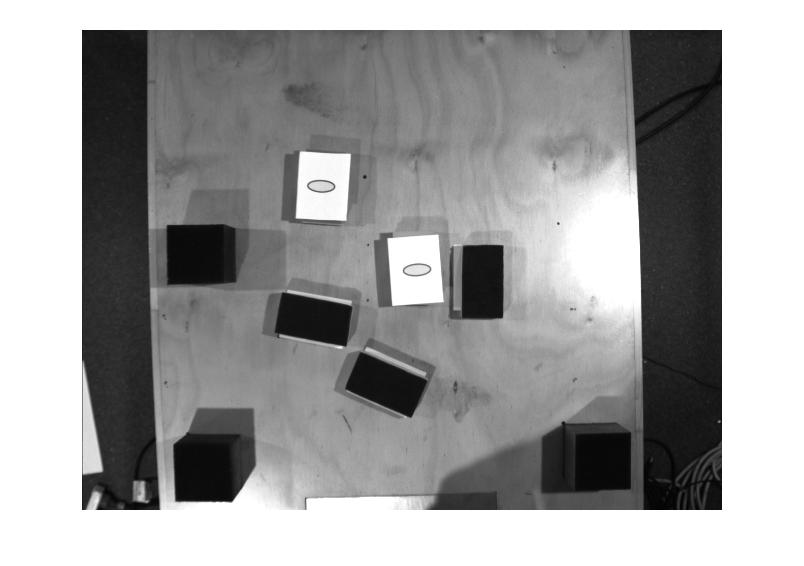
\includegraphics[scale=0.3]{./sachiths_images/image3.png}\\
		\caption[]{\textit{Initial captured image}}
	\end{centering}
\end{figure}

\begin{figure}[position = here]
	\begin{centering}
		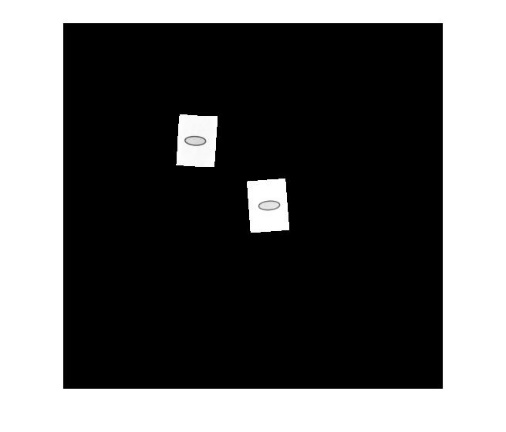
\includegraphics[scale=0.9]{./sachiths_images/image32.png}\\
		\caption[]{\textit{Isolated Cards}}
	\end{centering}
\end{figure}

2.	Coordinates and Pose of the cards
\begin{itemize}
	\item Logical image created using above mentioned method has been used to find the local centroids and the orientations of the cards. The function; regionprops has been used to find the centroids and orientation. After finding both, centroids and orientations of the fiducials have been removed. In orientations a redundancy has been added to make sure that the robot arm will always work in the safety limits by checking the value of the angle.
	
\end{itemize}

3.	Match the local coordinates to the world coordinates
\begin{itemize}
	\item 3 fiducials have been used to get the relative position of the cards. The method used was the perpendicular distance from two fiducials to the centroid of the card. Following figure will illustrate the method.
	
\end{itemize}
\begin{figure}[position = here]
	\begin{centering}
		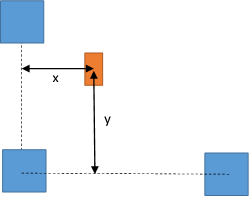
\includegraphics[scale=0.8]{./sachiths_images/image4.png}\\
		\caption[]{\textit{Method used to match with world coordinates}}
	\end{centering}
\end{figure}

4.	Identify the features of the cards
\begin{itemize}
	\item The main target was to identify the card itself before trying to extract features. Used the same method as above and identify the card using pixel values as thresholds. Used the found logical image as a mask to isolate only the card face.

\end{itemize}
\begin{figure}[position = here]
	\begin{centering}
		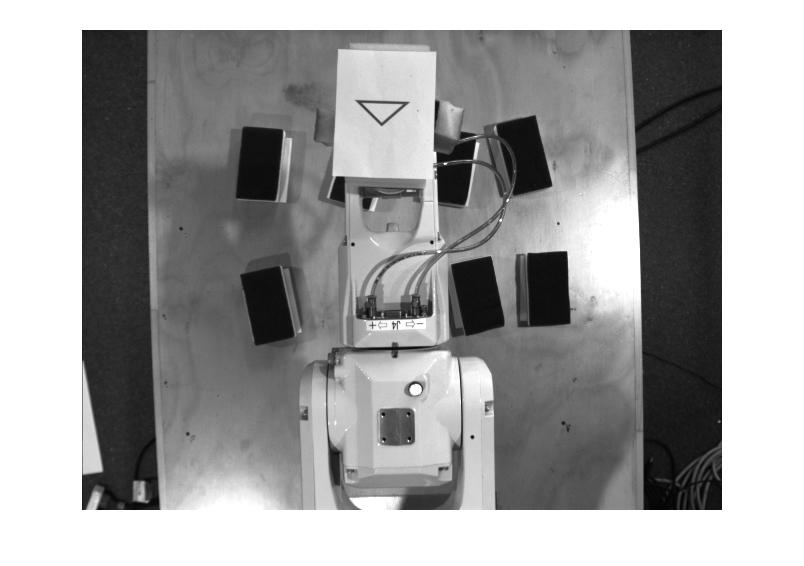
\includegraphics[scale=0.3]{./sachiths_images/image5.png}\\
		\caption[]{\textit{Initial image of the faceup card\label{imFup1}}}
	\end{centering}
\end{figure}
\begin{figure}[position = here]
	\begin{centering}
		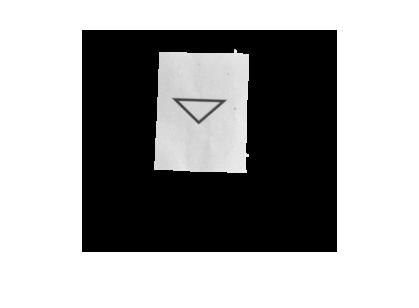
\includegraphics[scale=0.5]{./sachiths_images/image6.png}\\
		\caption[]{\textit{Isolated Card\label{isol1}}}
	\end{centering}
\end{figure}

\begin{itemize}
	\item From this image using a bounding box cropped out the card to process to find the features of shape, shape count and filler.
\end{itemize}

\begin{itemize}
	\item Edge detection has been used to find the shape. After detecting the edges of the shape unnecessary edges has been removed using clearing edges connected to border and removing connected regions less than a threshold pixel area.
	
\end{itemize}
\begin{figure}[position = here]
	\begin{centering}
		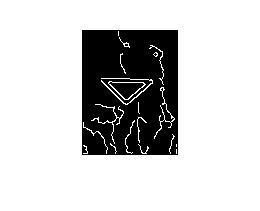
\includegraphics[scale=0.8]{./sachiths_images/image10.jpg}\\
		\caption[]{\textit{Identified Edges}}
	\end{centering}
\end{figure}
\begin{figure}[position = here]
	\begin{centering}
		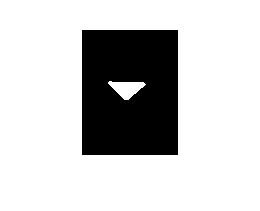
\includegraphics[scale=0.8]{./sachiths_images/image11.jpg}\\
		\caption[]{\textit{Identified Shape}}
	\end{centering}
\end{figure}
\begin{itemize}
	\item Perimeter of the founded blob has been used to identify the shape as triangle, rectangle and ellipse had different perimeter values. No of connected components in this stage has been used to identify the shape count. If the shape count is greater than 1, the mean perimeter will be checked for identify the shape. The final logical image with the shape has been used with the original image to identify the filler status. Mean intensity of the blob area of the logical image in original image will have a value greater than 0.72 if the shape is not shaded as pixel value for white is 1. For block status the mean intensity will be lowest and for shaded status the intensity value will be between 0.72 and 0.5.
	
	
\end{itemize}
	